\section*{Supporting Information}

\subsection*{Entity relationship diagram}
\begin{figure}
\begin{center}
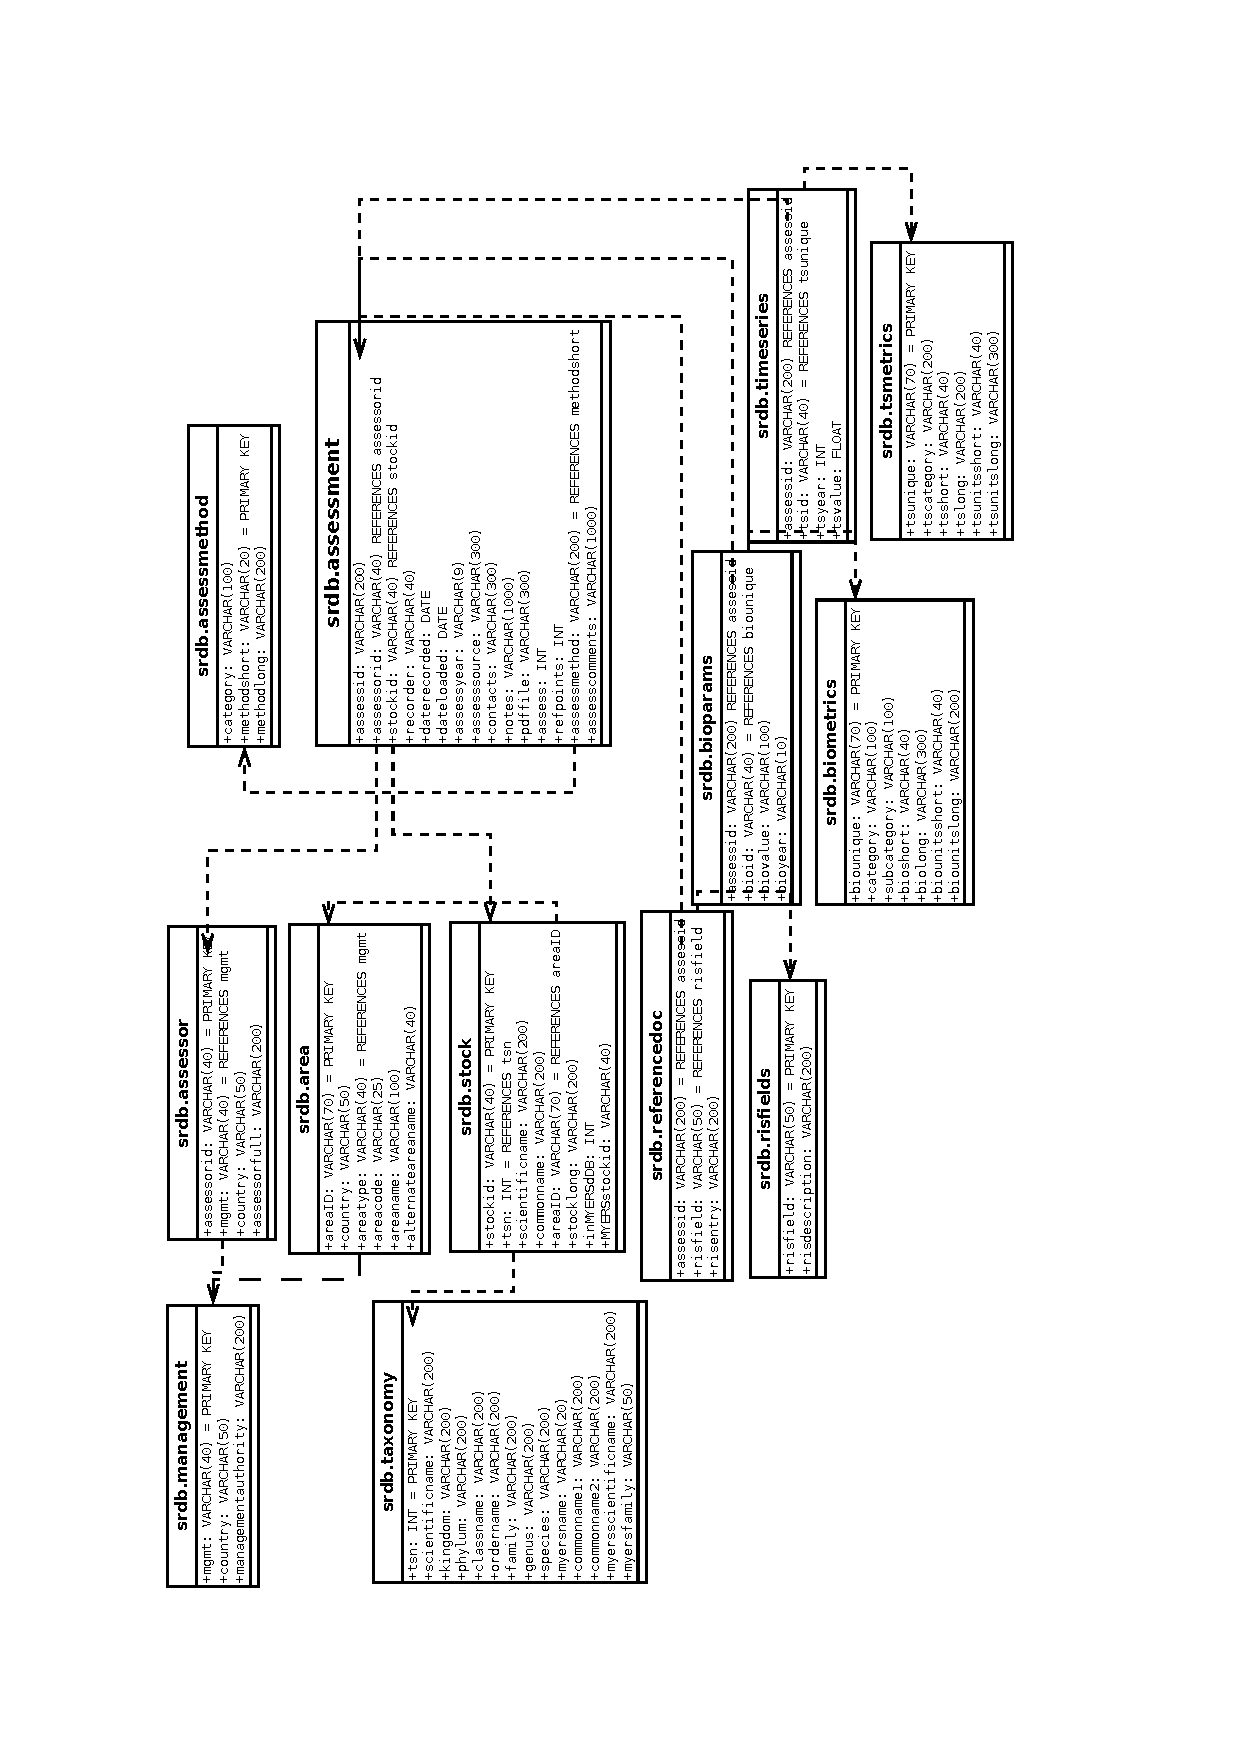
\includegraphics[width=15cm]{/home/srdbadmin/SQLpg/srdb/trunk/doc/srdb-ERD.pdf}
\end{center}
\caption{Entity relationship diagram of the RAM legacy database.}
\end{figure}


\begin{table}
\caption{Data used to generate Figure~\ref{fig:orca} - Summary of the assessments used in this analysis and the timespan of their different results. }
\begin{tabular}{| p{5cm} | p{3cm} | c | r  c  l | c | }\label{tab:timespan}
\textit{Fisheries stock} & \textit{Scientific name} & \textit{Timespan} & & \textit{Num. years available} & & \textit{Source} \\
 & & & Catch & SSB & R & \\
\hline \hline
blah & blah & 1970-2000 & 30 & 29 & 30 & (blah) \\
\end{tabular}
\end{table}


%\begin{table}
%\caption{Data used to generate Figures~\ref{fig:friedegg} and ~\ref{fig:friedeggmgmt} - Summary of the assessments used in this analysis and their estimated ratios of current biomass to the biomass at maximum sustainable yield and current harvest rate to the harvest rate that results is maximum sustainable yield. The estimated ratios were preferentially obtained directly from the assessment document or derived from surplus production model fits. When both an SSBmsy and Bmsy reference points are available, the SSB is chosen preferentially. }
%\begin{tabular}{| p{5cm} | p{3cm} | c | c | c | c | c |}\label{tab:crosshair}
%\textit{Fisheries stock} & \textit{Scientific name} & \textit{Current year} & \textit{B/Bmsy} & \textit{u/umsy} & \textit{From assessment?} & \textit{Source} \\
%\hline \hline
%blah & blah & 2000 & 1.0 & 1.0 & yes &  (blah) \\
%\end{tabular}
%\end{table}

% latex table generated in R 2.13.0 by xtable 1.5-6 package
% Thu May 19 14:38:14 2011
\begin{table}[ht]
\begin{center}
\begin{tabular}{ccc}
  \hline
 & SP U/Umsy $<$ 1 & SP U/Umsy $>$ 1 \\ 
  \hline
U/Umsy $<$ 1 &  20 &  14 \\ 
  U/Umsy $>$ 1 &   2 &   8 \\ 
  B/Bmsy $<$ 1 &  28 &   6 \\ 
  B/Bmsy $>$ 1 &  12 &  30 \\ 
   \hline
\end{tabular}
\caption{Contingency tables of stock status classification for biomass and exploitation reference points obtained from assessments and those derived from surplus production models. }
\label{tab:contingency}
\end{center}
\end{table}

\begin{table}[ht]
\begin{center}
\begin{tabular}{rllrrrl}
  \hline
 & stock & scientificname & currentyear & Bratio & Uratio & fromassessment \\
  \hline
1 & Alaska plaice Bering Sea and Aleutian Islands & Pleuronectes quadrituberculatus & 2008 & 2.46 & 0.05 & yes \\
  2 & Arrowtooth flounder Bering Sea and Aleutian Islands & Reinhardtius stomias & 2008 & 1.28 & 0.31 & no \\
  3 & Arrowtooth flounder Gulf of Alaska & Reinhardtius stomias & 2007 & 1.33 & 0.28 & no \\
  4 & Atka mackerel Bering Sea and Aleutian Islands & Pleurogrammus monopterygius & 2008 & 1.50 & 0.55 & no \\
  5 & Cabezon Northern California & Scorpaenichthys marmoratus & 2004 & 0.89 & 0.99 & no \\
  6 & Cabezon Southern California & Scorpaenichthys marmoratus & 2004 & 0.81 & 0.53 & no \\
  7 & Dusky rockfish Gulf of Alaska & Sebastes variabilis & 2007 & 1.54 & 0.54 & yes \\
  8 & Flathead sole Bering Sea and Aleutian Islands & Hippoglossoides elassodon & 2008 & 1.66 & 0.18 & no \\
  9 & Greenland turbot Bering Sea and Aleutian Islands & Reinhardtius hippoglossoides & 2009 & 1.48 & 0.05 & yes \\
  10 & Northern rockfish Bering Sea and Aleutian Islands & Sebastes polyspinis & 2008 & 1.07 & 0.13 & no \\
  11 & Northern rockfish Gulf of Alaska & Sebastes polyspinis & 2008 & 1.50 & 0.66 & yes \\
  12 & Northern rock sole Eastern Bering Sea and Aleutian Islands & Lepidopsetta polyxystra & 2007 & 3.02 & 0.21 & yes \\
  13 & Pacific cod Bering Sea and Aleutian Islands & Gadus macrocephalus & 2007 & 0.89 & 0.93 & no \\
  14 & Pacific cod Gulf of Alaska & Gadus macrocephalus & 2007 & 1.07 & 0.84 & no \\
  15 & Pacific Ocean perch Eastern Bering Sea and Aleutian Islands & Sebastes alutus & 2008 & 1.70 & 0.26 & no \\
  16 & Pacific ocean perch Gulf of Alaska & Sebastes alutus & 2008 & 1.16 & 0.73 & yes \\
  17 & Red king crab Bristol Bay & Paralithodes camtschaticus & 2007 & 0.00 & 1.38 & no \\
  18 & Sablefish Eastern Bering Sea / Aleutian Islands / Gulf of Alaska & Anoplopoma fimbria & 2008 & 0.72 & 0.90 & no \\
  19 & Snow crab Bering Sea & Chionoecetes opilio & 2008 & 0.29 & 1.61 & no \\
  20 & Walleye pollock Aleutian Islands & Theragra chalcogramma & 2008 & 0.86 & 0.02 & yes \\
  21 & Walleye pollock Eastern Bering Sea & Theragra chalcogramma & 2008 & 0.68 & 0.85 & no \\
  22 & Yellowfin sole Bering Sea and Aleutian Islands & Limanda aspera & 2008 & 1.94 & 0.62 & yes \\
  23 & Capelin Barents Sea & Mallotus villosus & 2006 & 0.17 & 0.00 & no \\
  24 & Atlantic cod coastal Norway & Gadus morhua & 2006 & 0.20 & 2.57 & no \\
  25 & Atlantic cod Northeast Arctic & Gadus morhua & 2006 & 0.56 & 1.42 & no \\
  26 & Greenland halibut Northeast Arctic & Reinhardtius hippoglossoides & 2006 & 0.23 & 1.38 & no \\
  27 & Golden Redfish Northeast Arctic & Sebastes norvegicus & 2006 & 0.00 & 4.25 & no \\
  28 & Haddock Northeast Arctic & Melanogrammus aeglefinus & 2006 & 1.10 & 1.06 & no \\
  29 & Pollock Northeast Arctic & Pollachius virens & 2006 & 1.70 & 0.60 & no \\
  30 & Atlantic croaker Mid-Atlantic Coast & Micropogonias undulatus & 2002 & 1.42 & 0.27 & yes \\
  31 & Northern shrimp Gulf of Maine & Pandalus borealis & 2008 & 1.58 & 0.56 & no \\
  32 & Antarctic toothfish Ross Sea & Dissostichus mawsoni & 2007 & 1.76 & 1.09 & no \\
  33 & Deepwater flathead Southeast Australia & Platycephalus conatus & 2006 & 1.33 & 0.61 & no \\
  34 & common gemfish Southeast Australia & Rexea solandri & 2007 & 0.01 & 0.59 & no \\
  35 & Jackass morwong Southeast Australia & Nemadactylus macropterus & 2007 & 0.25 & 1.80 & no \\
  36 & New Zealand ling Eastern half of Southeast Australia & Genypterus blacodes & 2007 & 0.60 & 2.20 & no \\
  37 & Orange roughy Cascade Plateau & Hoplostethus atlanticus & 2006 & 1.76 & 0.34 & no \\
  38 & Orange roughy Southeast Australia & Hoplostethus atlanticus & 2006 & 0.89 & 0.29 & no \\
  39 & Silverfish Southeast Australia & Seriolella punctata & 2006 & 1.15 & 0.79 & no \\
  40 & School whiting Southeast Australia & Sillago flindersi & 2007 & 1.10 & 0.82 & no \\
  41 & Tiger flathead Southeast Australia & Neoplatycephalus richardsoni & 2006 & 1.05 & 0.00 & no \\
  42 & Blue Warehou Eastern half of Southeast Australia & Seriolella brama & 2006 & 0.17 & 0.84 & no \\
  43 & Blue Warehou Western half of Southeast Australia & Seriolella brama & 2006 & 0.62 & 2.04 & no \\
  44 & Atlantic cod NAFO 5Zjm & Gadus morhua & 2002 & 0.00 & 0.74 & no \\
  45 & Haddock NAFO-4X5Y & Melanogrammus aeglefinus & 2003 & 0.28 & 0.45 & no \\
  46 & Haddock NAFO-5Zejm & Melanogrammus aeglefinus & 2002 & 0.15 & 0.86 & no \\
  47 & Atlantic cod NAFO 2J3KL inshore & Gadus morhua & 2005 & 1.60 & 0.14 & no \\
  48 & Atlantic cod NAFO 3Ps & Gadus morhua & 2004 & 0.43 & 0.43 & no \\
  49 & English sole Hecate Strait & Parophrys vetulus & 2001 & 1.23 & 0.37 & no \\
  50 & Pacific herring Central Coast & Clupea pallasii & 2007 & 0.30 & 0.11 & no \\
  51 & Pacific herring Prince Rupert District & Clupea pallasii & 2007 & 0.00 & 0.44 & no \\
  52 & Pacific herring Queen Charlotte Islands & Clupea pallasii & 2007 & 0.20 & 0.00 & no \\
  53 & Pacific herring Straight of Georgia & Clupea pallasii & 2007 & 0.91 & 0.40 & no \\
  54 & Pacific herring West Coast of Vancouver Island & Clupea pallasii & 2007 & 0.03 & 0.00 & no \\
  55 & Pacific cod Hecate Strait & Gadus macrocephalus & 2004 & 0.37 & 0.25 & no \\
  56 & Pacific cod West Coast of Vancouver Island & Gadus macrocephalus & 2001 & 0.28 & 0.61 & no \\
  57 & Rock sole Hecate Strait & Lepidopsetta bilineata & 2001 & 1.03 & 0.45 & no \\
  58 & Pollock NAFO-4VWX5Zc & Pollachius virens & 2006 & 0.56 & 0.30 & no \\
  59 & Atlantic cod NAFO 3Pn4RS & Gadus morhua & 2006 & 0.03 & 1.09 & no \\
  60 & Atlantic cod NAFO 4TVn & Gadus morhua & 2006 & 0.17 & 0.32 & no \\
  61 & Herring ICES 22-24-IIIa & Clupea harengus & 2006 & 0.73 & 1.02 & no \\
  62 & Herring Northern Irish Sea & Clupea harengus & 2006 & 0.72 & 0.34 & no \\
  63 & Herring North Sea & Clupea harengus & 2006 & 0.65 & 1.32 & no \\
  64 & Herring ICES VIa & Clupea harengus & 2006 & 0.18 & 1.59 & no \\
  65 & Herring ICES VIa-VIIb-VIIc & Clupea harengus & 2000 & 0.50 & 1.04 & no \\
  66 & Albacore tuna North Atlantic & Thunnus alalunga & 2005 & 0.81 & 1.49 & yes \\
  67 & Bluefin tuna Eastern Atlantic & Thunnus thynnus & 2007 & 0.34 & 9.38 & yes \\
  68 & Bluefin tuna Western Atlantic & Thunnus thynnus & 2007 & 0.57 & 1.33 & yes \\
  69 & Bigeye tuna Atlantic & Thunnus obesus & 2005 & 0.90 & 0.86 & no \\
  70 & Skipjack tuna Eastern Atlantic & Katsuwonus pelamis & 2006 & 1.71 & 0.27 & no \\
  71 & Skipjack tuna Western Atlantic & Katsuwonus pelamis & 2006 & 1.72 & 0.27 & no \\
  72 & Swordfish Mediterranean Sea & Xiphias gladius & 2006 & 0.94 & 1.27 & yes \\
  73 & Swordfish North Atlantic & Xiphias gladius & 2005 & 1.03 & 0.82 & no \\
  74 & Swordfish South Atlantic & Xiphias gladius & 2005 & 1.18 & 0.69 & no \\
  75 & Yellowfin tuna Atlantic & Thunnus albacares & 2006 & 1.07 & 0.81 & yes \\
  76 & Chilean jack mackerel Chilean EEZ and offshore & Trachurus murphyi & 2006 & 0.52 & 1.20 & no \\
  77 & Argentine anchoita Northern Argentina & Engraulis anchoita & 2007 & 1.37 & 0.17 & yes \\
  78 & Argentine anchoita Southern Argentina & Engraulis anchoita & 2007 & 3.13 & 0.04 & yes \\
  79 & Argentine hake Northern Argentina & Merluccius hubbsi & 2007 & 0.16 & 1.26 & yes \\
  80 & Argentine hake Southern Argentina & Merluccius hubbsi & 2008 & 0.34 & 1.49 & yes \\
  81 & Patagonian grenadier Southern Argentina & Macruronus magellanicus & 2006 & 1.82 & 0.60 & yes \\
  82 & Bigeye tuna Indian Ocean & Thunnus obesus & 2004 & 1.23 & 0.97 & yes \\
  83 & Pacific halibut North Pacific & Hippoglossus stenolepis & 2008 & 0.54 & 2.01 & no \\
  84 & Anchovy South Africa & Engraulis encrasicolus & 2006 & 0.97 & 0.36 & no \\
  85 & Shallow-water cape hake South Africa & Merluccius capensis & 2008 & 1.16 & 0.40 & no \\
  86 & Cape horse mackerel South Africa South coast & Trachurus capensis & 2007 & 1.47 & 0.76 & no \\
  87 & Kingklip South Africa & Engraulis encrasicolus & 2008 & 1.13 & 0.55 & no \\
  88 & Sardine South Africa & Sardinops sagax & 2006 & 0.75 & 0.55 & no \\
  89 & Southern spiny lobster South Africa South coast & Palinurus gilchristi & 2008 & 0.51 & 1.50 & no \\
  90 & American Plaice NAFO-3LNO & Hippoglossoides platessoides & 2006 & 0.02 & 1.05 & no \\
  91 & American Plaice NAFO-3M & Hippoglossoides platessoides & 2007 & 0.00 & 0.00 & no \\
  92 & Atlantic cod NAFO 3NO & Gadus morhua & 2006 & 0.00 & 0.38 & no \\
  93 & Greenland halibut NAFO 23KLMNO & Reinhardtius hippoglossoides & 2006 & 0.39 & 1.73 & no \\
  94 & Redfish species NAFO 3LN & Redfish species & 2008 & 1.88 & 0.04 & yes \\
  95 & Redfish species NAFO 3M & Redfish species & 2006 & 0.93 & 0.15 & no \\
  96 & Yellowtail Flounder NAFO 3LNO & Limanda ferruginea & 2007 & 1.62 & 0.15 & no \\
  97 & American Plaice NAFO-5YZ & Hippoglossoides platessoides & 2007 & 0.55 & 0.30 & no \\
  98 & Bluefish Atlantic Coast & Pomatomus saltatrix & 2007 & 0.81 & 1.25 & no \\
  99 & Black sea bass Mid-Atlantic Coast & Centropristis striata & 2007 & 1.21 & 0.67 & no \\
  100 & Atlantic cod Georges Bank & Gadus morhua & 2007 & 0.00 & 1.15 & no \\
  101 & Atlantic cod Gulf of Maine & Gadus morhua & 2007 & 1.46 & 0.29 & no \\
  102 & Haddock NAFO-5Y & Melanogrammus aeglefinus & 2007 & 0.00 & 1.86 & no \\
  103 & Monkfish Gulf of Maine / Northern Georges Bank & Lophius americanus & 2006 & 1.73 & 0.38 & no \\
  104 & Monkfish Southern Georges Bank / Mid-Atlantic & Lophius americanus & 2006 & 1.72 & 0.30 & no \\
  105 & Sea scallop Georges Bank & Placopecten magellanicus & 2006 & 1.59 & 0.78 & no \\
  106 & Sea scallop Mid-Atlantic Coast & Placopecten magellanicus & 2006 & 0.91 & 0.37 & no \\
  107 & Spiny dogfish Atlantic Coast & Squalus acanthias & 2005 & 1.61 & 0.15 & no \\
  108 & Atlantic surfclam Mid-Atlantic Coast & Spisula solidissima & 1994 & 1.85 & 0.00 & no \\
  109 & Tilefish Mid-Atlantic Coast & Lopholatilus chamaeleonticeps & 2005 & 0.72 & 0.61 & no \\
  110 & Weakfish Atlantic Coast & Cynoscion regalis & 2008 & 0.06 & 1.49 & no \\
  111 & White hake Georges Bank / Gulf of Maine & Urophycis tenuis & 2007 & 0.35 & 0.80 & yes \\
  112 & Winter Flounder NAFO-5Z & Pseudopleuronectes americanus & 2006 & 1.41 & 0.25 & no \\
  113 & Winter Flounder Southern New England-Mid Atlantic & Pseudopleuronectes americanus & 2007 & 0.07 & 1.44 & no \\
  114 & Witch Flounder NAFO-5Y & Glyptocephalus cynoglossus & 2007 & 0.30 & 1.45 & yes \\
  115 & Yellowtail flounder Cape Cod / Gulf of Maine & Limanda ferruginea & 2007 & 0.25 & 1.73 & yes \\
  116 & Yellowtail flounder Georges Bank & Limanda ferruginea & 2007 & 0.22 & 1.14 & yes \\
  117 & Yellowtail Flounder Southern New England-Mid Atlantic & Limanda ferruginea & 2007 & 0.13 & 1.61 & yes \\
  118 & Australian salmon New Zealand & Arripis trutta & 2006 & 1.64 & 0.33 & yes \\
  119 & Orange roughy New Zealand Mid East Coast & Hoplostethus atlanticus & 2004 & 1.20 & 0.35 & yes \\
  120 & Atlantic menhaden Atlantic & Brevoortia tyrannus & 2005 & 0.47 & 0.97 & no \\
  121 & Pacific sardine North Pacific & Sardinops sagax & 2006 & 1.73 & 0.37 & no \\
  122 & Arrowtooth flounder Pacific Coast & Reinhardtius stomias & 2007 & 3.81 & 0.21 & yes \\
  123 & Blackgill rockfish  Pacific Coast & Sebastes melanostomus & 2004 & 0.80 & 1.20 & no \\
  124 & Black rockfish Northern Pacific Coast & Sebastes melanops & 2006 & 1.37 & 0.57 & no \\
  125 & Black rockfish Southern Pacific Coast & Sebastes melanops & 2007 & 2.23 & 0.33 & yes \\
  126 & Blue rockfish California & Sebastes mystinus & 2007 & 0.75 & 1.19 & yes \\
  127 & Bocaccio Southern Pacific Coast & Sebastes paucispinis & 2006 & 0.32 & 0.10 & yes \\
  128 & Chilipepper Southern Pacific Coast & Sebastes goodei & 2006 & 1.43 & 0.04 & no \\
  129 & Cowcod Southern California & Sebastes levis & 2007 & 0.09 & 0.07 & yes \\
  130 & Canary rockfish Pacific Coast & Sebastes pinniger & 2007 & 0.85 & 0.02 & yes \\
  131 & Darkblotched rockfish Pacific Coast & Sebastes crameri & 2007 & 0.73 & 0.31 & yes \\
  132 & English sole Pacific Coast & Parophrys vetulus & 2006 & 2.06 & 0.14 & no \\
  133 & Longnose skate Pacific Coast & Raja rhina & 2007 & 1.56 & 0.40 & no \\
  134 & Longspine thornyhead Pacific Coast & Sebastolobus altivelis & 2005 & 2.65 & 0.23 & yes \\
  135 & Pacific hake Pacific Coast & Merluccius productus & 2007 & 0.42 & 1.67 & no \\
  136 & Pacific ocean perch Pacific Coast & Sebastes alutus & 2007 & 0.69 & 0.00 & yes \\
  137 & Petrale sole Northern Pacific Coast & Eopsetta jordani & 2004 & 0.96 & 1.26 & no \\
  138 & Petrale sole Southern Pacific Coast & Eopsetta jordani & 2004 & 0.63 & 0.61 & no \\
  139 & Sablefish Pacific Coast & Anoplopoma fimbria & 2007 & 0.84 & 1.09 & no \\
  140 & Shortspine thornyhead Pacific Coast & Sebastolobus alascanus & 2004 & 1.55 & 0.93 & no \\
  141 & Widow rockfish Pacific Coast & Sebastes entomelas & 2006 & 0.91 & 0.07 & no \\
  142 & Yelloweye rockfish Pacific Coast & Sebastes ruberrimus & 2006 & 0.38 & 0.34 & no \\
  143 & Yellowtail rockfish Northern Pacific Coast & Sebastes flavidus & 2005 & 0.75 & 0.51 & no \\
  144 & Capelin Iceland & Mallotus villosus & 2006 & 0.49 & 0.85 & no \\
  145 & Atlantic cod Faroe Plateau & Gadus morhua & 2006 & 0.26 & 1.52 & no \\
  146 & Atlantic cod Iceland & Gadus morhua & 2006 & 0.46 & 1.17 & no \\
  147 & Haddock Faroe Plateau & Melanogrammus aeglefinus & 2006 & 0.85 & 1.07 & no \\
  148 & Haddock Iceland & Melanogrammus aeglefinus & 2007 & 0.73 & 1.36 & no \\
  149 & Pollock Faroe Plateau & Pollachius virens & 2006 & 0.99 & 1.52 & no \\
  150 & Black oreo West end of Chatham Rise & Allocyttus niger & 2007 & 0.99 & 0.82 & yes \\
  151 & Smooth oreo Chatham Rise & Pseudocyttus maculatus & 2006 & 2.25 & 0.38 & yes \\
  152 & Smooth oreo West end of Chatham Rise & Pseudocyttus maculatus & 2004 & 1.25 & 0.53 & yes \\
  153 & Hoki Eastern New Zealand & Macruronus novaezelandiae & 2007 & 1.11 & 0.33 & no \\
  154 & Hoki Western New Zealand & Macruronus novaezelandiae & 2007 & 0.51 & 0.57 & no \\
  155 & New Zealand snapper New Zealand Area 8 & Chrysophrys auratus & 2005 & 0.35 & 2.50 & yes \\
  156 & Trevally New Zealand Areas TRE 7 & Pseudocaranx dentex & 2005 & 1.44 & 0.83 & yes \\
  157 & Red rock lobster New Zealand area CRA1 & Jasus edwardsii & 2001 & 1.14 & 0.88 & no \\
  158 & Red rock lobster New Zealand area CRA2 & Jasus edwardsii & 2001 & 0.53 & 2.12 & no \\
  159 & Red rock lobster New Zealand area CRA4 & Jasus edwardsii & 2005 & 0.67 & 1.33 & no \\
  160 & Red rock lobster New Zealand area CRA5 & Jasus edwardsii & 2002 & 0.59 & 1.68 & no \\
  161 & Red rock lobster New Zealand area CRA7 & Jasus edwardsii & 2005 & 0.73 & 0.43 & no \\
  162 & Red rock lobster New Zealand area CRA8 & Jasus edwardsii & 2005 & 0.69 & 0.49 & no \\
  163 & common gemfish New Zealand & Rexea solandri & 2006 & 1.64 & 0.43 & yes \\
  164 & New Zealand ling New Zealand Areas LIN 3 and 4 & Genypterus blacodes & 2007 & 3.07 & 0.09 & yes \\
  165 & New Zealand ling New Zealand Areas LIN 5 and 6 & Genypterus blacodes & 2007 & 3.96 & 0.10 & yes \\
  166 & New Zealand ling New Zealand Area LIN 6b & Genypterus blacodes & 2006 & 2.19 & 0.11 & yes \\
  167 & New Zealand ling New Zealand Area LIN 72 & Genypterus blacodes & 2007 & 2.49 & 0.32 & yes \\
  168 & New Zealand ling New Zealand Area LIN 7WC - WCSI & Genypterus blacodes & 2008 & 2.21 & 0.13 & yes \\
  169 & Southern blue whiting Campbell Island Rise & Micromesistius australis & 2006 & 1.15 & 0.92 & yes \\
  170 & Southern hake Chatham Rise & Merluccius australis & 2006 & 1.77 & 0.12 & yes \\
  171 & Southern hake Sub-Antarctic & Merluccius australis & 2007 & 2.91 & 0.11 & yes \\
  172 & New Zealand abalone species New Zealand Area PAU 5A & Haliotis iris & 2006 & 0.72 & 2.83 & no \\
  173 & New Zealand abalone species New Zealand Area PAU 5B & Haliotis iris & 2007 & 1.02 & 0.59 & no \\
  174 & New Zealand abalone species New Zealand Area PAU 5D & Haliotis iris & 2006 & 0.44 & 2.10 & no \\
  175 & New Zealand abalone species New Zealand Area PAU 7 & Haliotis iris & 2008 & 0.87 & 0.94 & no \\
  176 & American lobster Rhode Island & Homarus americanus & 2006 & 0.51 & 0.68 & no \\
  177 & Tautog Rhode Island & Tautoga onitis & 2006 & 0.84 & 0.59 & no \\
  178 & Winter flounder Rhode Island & Pseudopleuronectes americanus & 2006 & 0.03 & 2.35 & no \\
  179 & Gag Gulf of Mexico & Mycteroperca microlepis & 2004 & 1.25 & 1.84 & no \\
  180 & Gag Southern Atlantic coast & Mycteroperca microlepis & 2005 & 0.94 & 1.31 & yes \\
  181 & Greater amberjack Gulf of Mexico & Seriola dumerili & 2004 & 0.46 & 1.52 & no \\
  182 & King mackerel Gulf of Mexico & Scomberomorus cavalla & 2001 & 1.51 & 0.44 & no \\
  183 & King mackerel Southern Atlantic Coast & Scomberomorus cavalla & 2001 & 1.38 & 0.56 & no \\
  184 & Gulf menhaden Gulf of Mexico & Brevoortia patronus & 2004 & 1.08 & 0.48 & no \\
  185 & Red grouper Gulf of Mexico & Epinephelus morio & 2005 & 0.17 & 1.39 & no \\
  186 & Red porgy Southern Atlantic coast & Pagrus pagrus & 2004 & 0.61 & 0.39 & yes \\
  187 & Snowy grouper Southern Atlantic coast & Epinephelus niveatus & 2002 & 0.19 & 3.08 & yes \\
  188 & Spanish mackerel Southern Atlantic Coast & Scomberomorus maculatus & 2007 & 0.38 & 0.91 & yes \\
  189 & Tilefish Southern Atlantic coast & Lopholatilus chamaeleonticeps & 2002 & 0.94 & 1.55 & yes \\
  190 & Vermilion snapper Southern Atlantic coast & Rhomboplites aurorubens & 2007 & 0.86 & 1.27 & yes \\
  191 & Yellowtail snapper Southern Atlantic Coast and Gulf of Mexico & Ocyurus chrysurus & 2001 & 1.14 & 0.61 & yes \\
  192 & Walleye pollock Northern Sea of Okhotsk & Theragra chalcogramma & 1992 & 1.11 & 0.87 & no \\
  193 & Albacore tuna South Pacific Ocean & Thunnus alalunga & 2006 & 2.46 & 0.90 & yes \\
  194 & Bigeye tuna Western Pacific Ocean & Thunnus obesus & 2006 & 1.06 & 1.38 & yes \\
  195 & Skipjack tuna Central Western Pacific & Katsuwonus pelamis & 2006 & 4.38 & 0.30 & yes \\
  196 & Yellowfin tuna Central Western Pacific & Thunnus albacares & 2005 & 1.22 & 0.80 & yes \\
  197 & Dover sole Pacific Coast & Microstomus pacificus & 2004 & 1.33 & 0.45 & no \\
  198 & Gopher rockfish Southern Pacific Coast & Sebastes carnatus & 2004 & 1.69 & 0.08 & no \\
  199 & Pacific sardine Pacific Coast & Sardinops sagax & 2006 & 1.36 & 0.41 & no \\
  200 & Starry flounder Northern Pacific Coast & Platichthys stellatus & 2004 & 0.68 & 0.33 & no \\
  201 & Starry flounder Southern Pacific Coast & Platichthys stellatus & 2004 & 1.15 & 0.12 & no \\
  202 & Tasmanian giant crab Tasmania & Pseudocarcinus gigas & 2007 & 0.50 & 1.71 & no \\
  203 & Walleye pollock Western Bering Sea & Theragra chalcogramma & 2004 & 2.16 & 0.26 & no \\
  204 & Atlantic cod Baltic Areas 22 and 24 & Gadus morhua & 2006 & 0.31 & 1.55 & no \\
  205 & Atlantic cod Baltic Areas 25-32 & Gadus morhua & 2006 & 0.14 & 1.58 & no \\
  206 & Atlantic cod Kattegat & Gadus morhua & 2006 & 0.19 & 0.31 & no \\
  207 & Herring ICES 25-32 & Clupea harengus & 2006 & 0.69 & 0.79 & no \\
  208 & Herring ICES 30 & Clupea harengus & 2006 & 1.19 & 1.10 & no \\
  209 & Herring ICES 31 & Clupea harengus & 2006 & 0.27 & 1.65 & no \\
  210 & Herring Iceland (Summer spawners) & Clupea harengus & 2006 & 0.70 & 0.89 & no \\
  211 & Herring ICES 28 & Clupea harengus & 2006 & 1.21 & 0.87 & no \\
  212 & common European sole ICES Kattegat and Skagerrak & Solea vulgaris & 2006 & 1.25 & 0.54 & no \\
  213 & Sprat ICES Baltic Areas 22-32 & Sprattus sprattus & 2006 & 1.13 & 1.27 & no \\
  214 & Fourspotted megrim ICES VIIIc-IXa & Lepidorhombus boscii & 2006 & 0.00 & 1.61 & no \\
  215 & Hake Northeast Atlantic North & Merluccius merluccius & 2006 & 1.04 & 0.74 & no \\
  216 & Megrim ICES VIIIc-IXa & Lepidorhombus whiffiagonis & 2006 & 0.24 & 1.31 & no \\
  217 & common European sole Bay of Biscay & Solea vulgaris & 2006 & 0.62 & 1.13 & no \\
  218 & Mackerel ICES Northeast Atlantic & Scomber scombrus & 2006 & 0.98 & 0.73 & no \\
  219 & Whiting Northeast Atlantic & Micromesistius poutassou & 2006 & 0.67 & 1.66 & no \\
  220 & Atlantic cod Irish Sea & Gadus morhua & 2006 & 0.09 & 0.69 & no \\
  221 & Atlantic cod West of Scotland & Gadus morhua & 2006 & 0.10 & 0.45 & no \\
  222 & Haddock West of Scotland & Melanogrammus aeglefinus & 2006 & 0.58 & 0.73 & no \\
  223 & European Plaice Irish Sea & Pleuronectes platessa & 2006 & 1.07 & 0.23 & no \\
  224 & common European sole Irish Sea & Solea vulgaris & 2006 & 0.36 & 1.16 & no \\
  225 & Atlantic cod North Sea & Gadus morhua & 2006 & 0.19 & 0.80 & no \\
  226 & Haddock ICES IIIa and North Sea & Melanogrammus aeglefinus & 2006 & 0.62 & 0.25 & no \\
  227 & Haddock Rockall Bank & Melanogrammus aeglefinus & 2006 & 1.10 & 0.52 & no \\
  228 & Norway pout North Sea & Trisopterus esmarkii & 2006 & 0.90 & 0.33 & no \\
  229 & Pollock ICES IIIa, VI and North Sea & Pollachius virens & 2006 & 0.56 & 0.97 & no \\
  230 & Sandeel North Sea & Ammodytes marinus & 2007 & 0.92 & 0.24 & no \\
  231 & Whiting ICES IIIa, VIId and North Sea & Merlangius merlangus & 2006 & 0.33 & 1.04 & no \\
  232 & Haddock ICES VIIb-k & Melanogrammus aeglefinus & 2006 & 1.37 & 0.41 & no \\
  233 & European Plaice ICES VIIf-g & Pleuronectes platessa & 2006 & 0.65 & 0.41 & no \\
  234 & European Plaice ICES VIIe & Pleuronectes platessa & 2006 & 0.51 & 1.39 & no \\
  235 & common European sole Celtic Sea & Solea vulgaris & 2006 & 0.90 & 0.95 & no \\
  236 & common European sole Western English Channel & Solea vulgaris & 2006 & 0.51 & 1.75 & no \\
  237 & Whiting ICES VIIe-k & Merlangius merlangus & 2006 & 0.44 & 1.25 & no \\
   \hline
\end{tabular}
\caption{Data used to generate Figures~\ref{fig:friedegg} and ~\ref{fig:friedeggmgmt} - Summary of the assessments used in this analysis and their estimated ratios of current biomass to the biomass at maximum sustainable yield and current harvest rate to the harvest rate that results is maximum sustainable yield. The estimated ratios were preferentially obtained directly from the assessment document or derived from surplus production model fits. When both an SSBmsy and Bmsy reference points are available, the SSB is chosen preferentially.}
\label{tab:crosshair}
\end{center}
\end{table}
